% vim:encoding=utf8 ft=tex sts=2 sw=2 et:

\documentclass{classrep}
\usepackage[utf8x]{inputenc}
\usepackage[a4paper, left=1.5cm, right=1.5cm, top=1.0cm, bottom=1.5cm, headsep=0.5cm, headheight=13pt]{geometry}
\usepackage{amsmath, amsthm, amssymb, amsfonts}
\usepackage{graphicx}
\usepackage{float}
\usepackage{listings}

\lstdefinelanguage{VHDL}{
	morekeywords={
		library,use,all,entity,is,port,in,out,end,architecture,of,if,downto,process,when,then,elsif,
		begin,and,LIBRARY,USE,ALL,ENTITY,IS,PORT,IN,OUT,END,ARCHITECTURE,OF,BEGIN,AND
	},
	morecomment=[l]--
}

\usepackage{xcolor}
\colorlet{keyword}{blue!100!black!80}
\colorlet{comment}{green!90!black!90}
\lstdefinestyle{vhdl}{
	language     = VHDL,
	basicstyle   = \ttfamily,
	keywordstyle = \color{keyword}\bfseries,
	 stringstyle=\ttfamily\color{red!50!brown},
	commentstyle = \color{comment}
}
\lstset{language=VHDL,style=vhdl,literate=%
	*{0}{{{\color{red!20!violet}0}}}1
	{1}{{{\color{red!20!violet}1}}}1
	{2}{{{\color{red!20!violet}2}}}1
	{3}{{{\color{red!20!violet}3}}}1
	{4}{{{\color{red!20!violet}4}}}1
	{5}{{{\color{red!20!violet}5}}}1
	{6}{{{\color{red!20!violet}6}}}1
	{7}{{{\color{red!20!violet}7}}}1
	{8}{{{\color{red!20!violet}8}}}1
	{9}{{{\color{red!20!violet}9}}}1}

\usepackage{hyperref} % musi być na końcu
\hypersetup{pdfborder={0 0 0 0}}



\studycycle{Elektronika i Telekomunikacja, studia dzienne, mgr II st.}
\coursesemester{I}

\coursename{Programowalne układy cyfrowe}
\courseyear{2014/2015}

\courseteacher{mgr. Tomaszewski Grzegorz}
\coursegroup{poniedziałek, 14:00}

\author{
  \studentinfo{Witold Olechowski}{127517} \and
  \studentinfo{Tomasz Marecik}{127374}
}

\title{Zadanie 3,4: Projektowanie prostych układów kombinacyjnych z użyciem języka VHDL }

%\lstinputlisting{block1.vhdl}
%\vskip 2\baselineskip

\begin{document}
\maketitle

\section{Cel:}
\textbf{Używając języka VHDL zrealizować:}
\begin{itemize}
	\item transkoder kodu BCD 8421 na kod wskaźnika 7-segmentowego
	\item demultiplekser umożliwiający wybór 1 z 4 wyświetlaczy LED
\end{itemize}

\section{Pierwszy wariant realizacji zadania}

\begin{figure}[H]
	\centering
	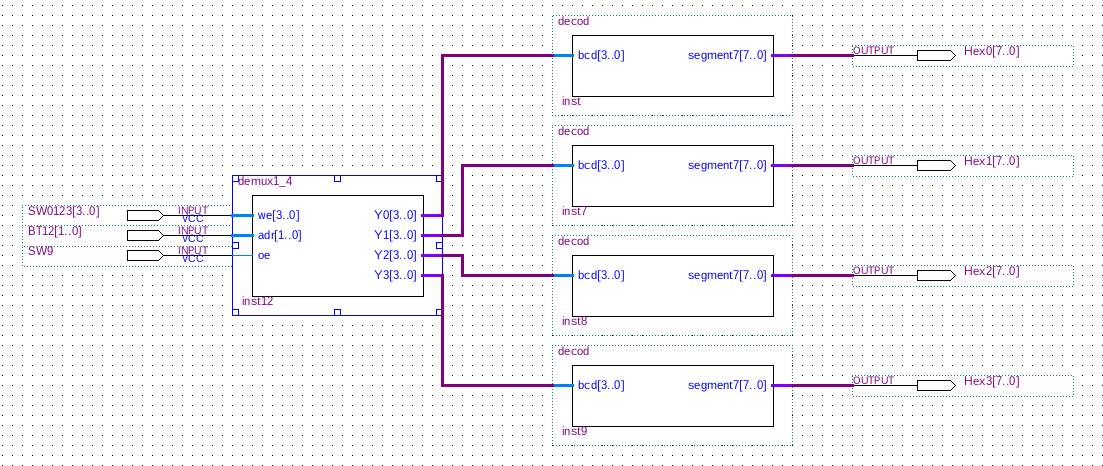
\includegraphics[width=1.0\linewidth]{block_bcd_segment}
	\caption{Schemat blokowy układu}
	\label{fig:block_bcd_segment}
\end{figure}

\subsection{Listing kodu źródłowego dla demultipleksera:}
	\lstinputlisting{demux1_4.vhd}

\subsection{Listing kodu źródłowego dla dekodera BCD:}
	\lstinputlisting{decod.vhd}

\subsection{Przebiegi czasowe układu:}

\begin{figure}[H]
	\centering
	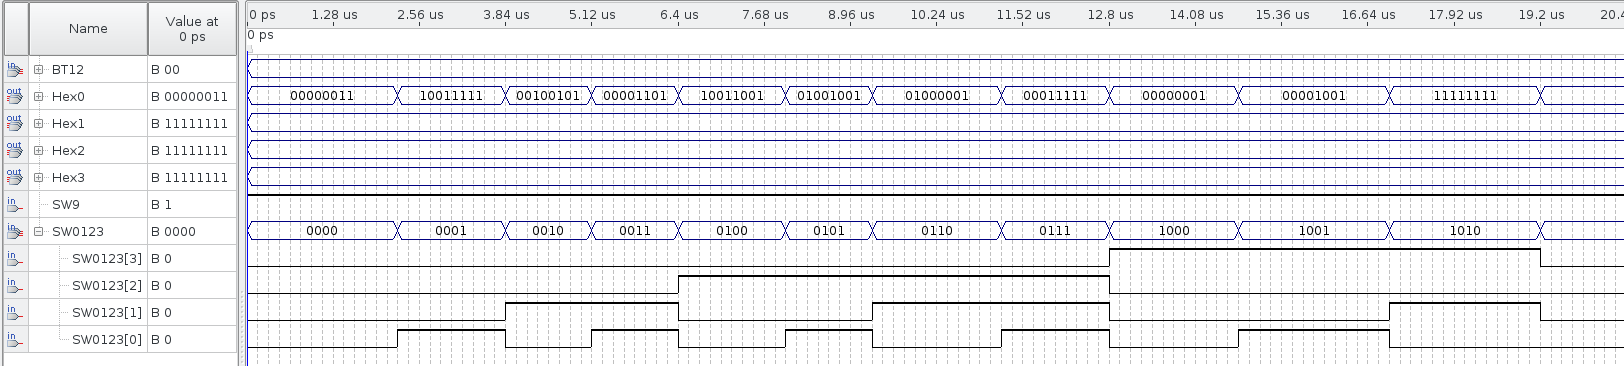
\includegraphics[width=1.0\linewidth]{symhex0}
	\caption{SW9='1', BT12='00'}
	\label{fig:symhex0}
\end{figure}
\begin{figure}[H]
	\centering
	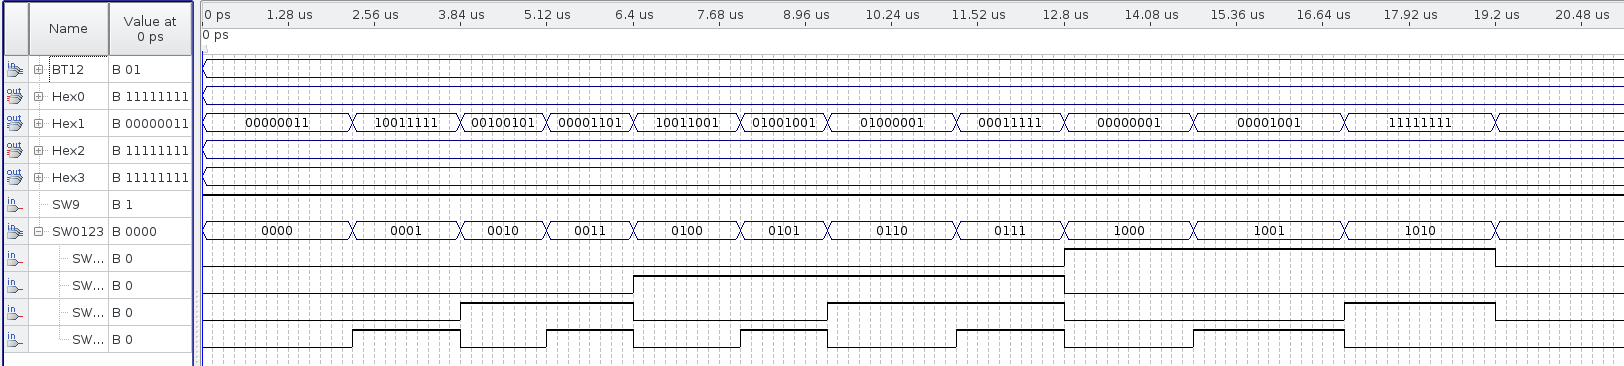
\includegraphics[width=1.0\linewidth]{symhex1}
	\caption{SW9='1', BT12='01'}
	\label{fig:symhex1}
\end{figure}

\begin{figure}[H]
	\centering
	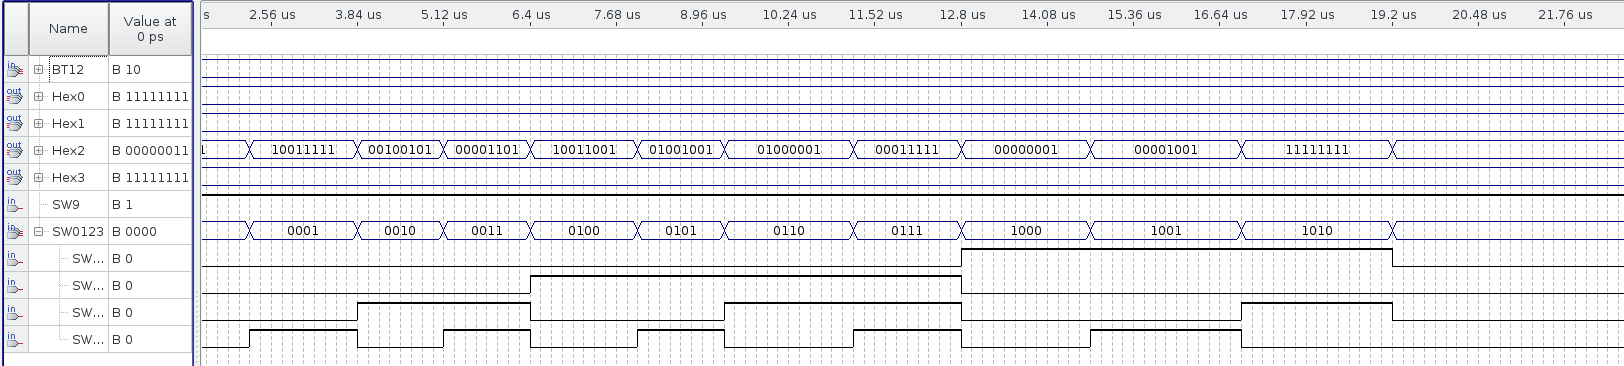
\includegraphics[width=1.0\linewidth]{symhex2}
	\caption{SW9='1', BT12='10'}
	\label{fig:symhex2}
\end{figure}

\begin{figure}[H]
	\centering
	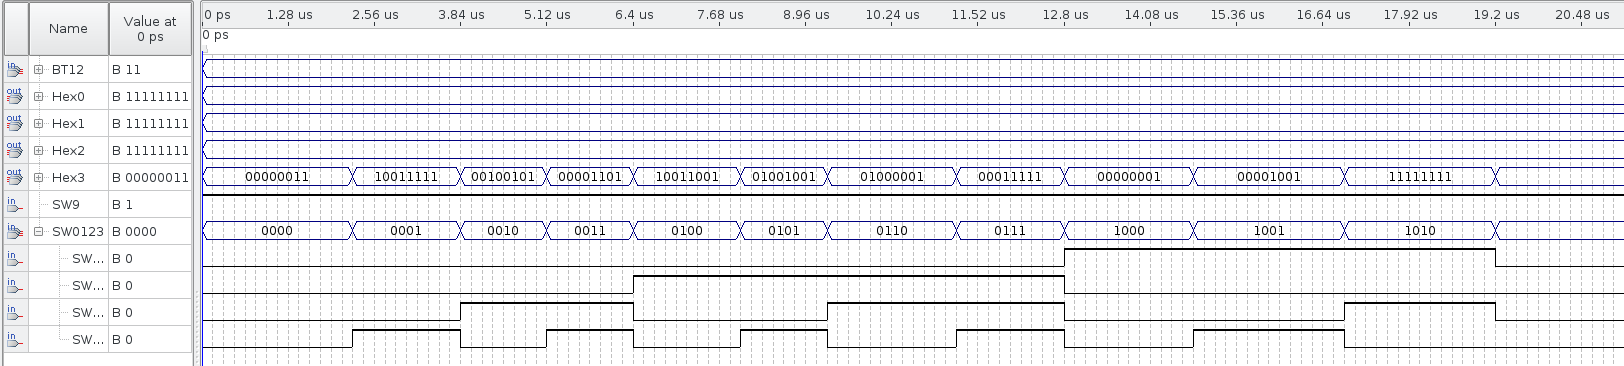
\includegraphics[width=1.0\linewidth]{symhex3}
	\caption{SW9='1', BT12='11'}
	\label{fig:symhex3}
\end{figure}

\begin{figure}[H]
	\centering
	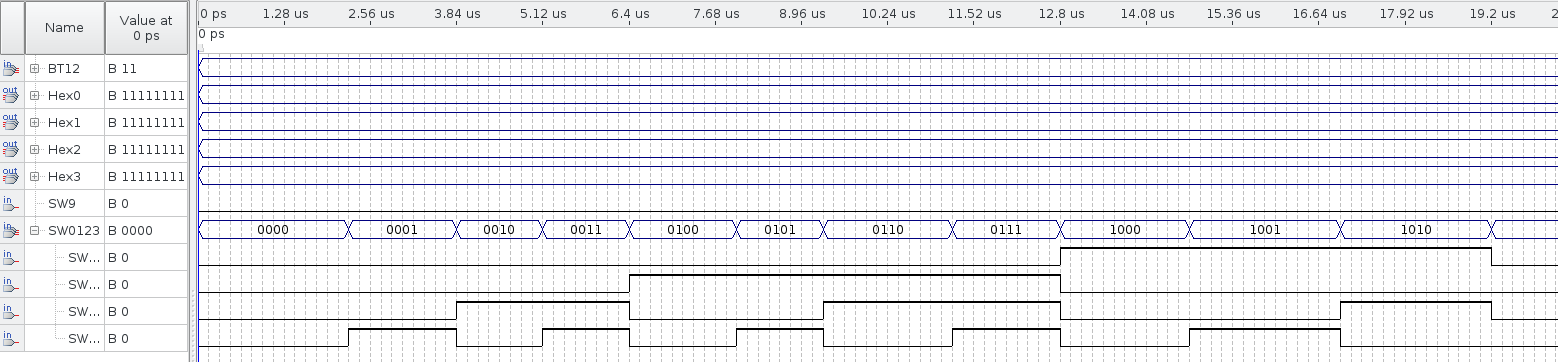
\includegraphics[width=1.0\linewidth]{symhex3not_oe}
	\caption{SW9='0', BT12='11'}
	\label{fig:symhex3not_oe}
\end{figure}

\section{Drugi wariant realizacji zadania z transkodowaniem}

\section{Wnioski}
\begin{itemize}
	\item 
\end{itemize}

\begin{thebibliography}{0}
  \bibitem{l2short} John Wiley and Sons Publishers.
    \textsl{Digital Design,} University of California, Riverside, 2007
\end{thebibliography}
\end{document}
